\documentclass[12pt]{article}
\usepackage{latexsym}
\usepackage{tikz}
\usetikzlibrary{automata,positioning}


\topmargin = 0.1in \textwidth=5.7in \textheight=8.6in

\oddsidemargin = 0.2in \evensidemargin = 0.2in


\begin{document}

\begin{center}
    Theory of Computation, SPRING 2015 \\
    Mid Term\\
    Author: Tawheed Abdul-Raheem\\
\end{center}

\smallskip

\begin{enumerate}
    \item Please provide an example of a regular expression, contating union, concatenation and  at least two occurrences of Klene star (*), draw or define a finite automaton corresponding to this expression.
    \[ (a \cup b^*)c^* \]
    
     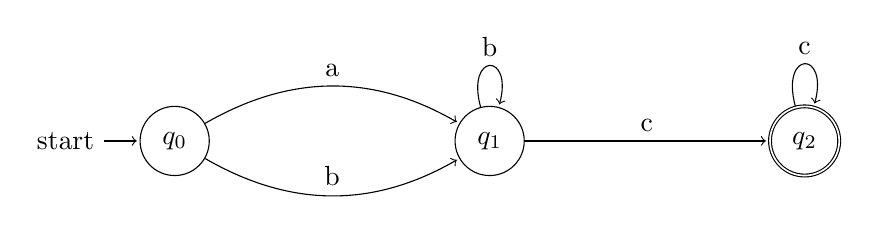
\begin{tikzpicture}[shorten >=1pt,node distance=4cm,on grid,auto] 
   \node[state,initial] (q_0)   {$q_0$}; 
   \node[state] (q_1) [ right=of q_0] {$q_1$};
   \node[state, accepting] (q_2) [ right=of q_1] {$q_2$};
    \path[->] 
    (q_0)
        edge [bend left] node {a} (q_1)
        edge [bend right] node {b} (q_1)

    (q_1) 
          edge  node {c} (q_2)
          edge [loop above] node {b} ()
          
    (q_2) 
      edge [loop above] node {c} ();
\end{tikzpicture}
    
    
    \item Please show that the language containing all strings of 1's and 0's except those strings that have equal number of of 1's and 0's is not regular.
    
    \[ \{1^n \: 0^n \: | \: n \: \in \: N \} \; is \; not \; regular\]
    
    \textbf{Proof:}
    \[ let \; L  \; = \; \{1^n \; 0^n \; | \; n \in N \}\]
    \[Assume \; L \; is  \; regular,  \;let  \; m  \;be \; the \; number \; from  \;the  \;pumping \; lemma \]
    \[ Let  \; s  \; =  \; 1^m  \; 0^m\]
    \[ Since  \;  s \; \in  \; L  \; and  \;|s|   \;\geq \; m \; the  \; lemma  \; must  \; apply,  \; specifically\]
    \[s  \; =  \; xyz  \; where  \; y  \;= \; \lambda  \; and  \; |xy| \leq m  \]
    \[ y  \; =  \; 1^k  \; where  \;  \; 0  \; <  \; k \leq m\]
    \[x  \; =  \; 1^q  \; where  \;  \; 0 \leq  \;q  \;< \; m \]
    \[z  \; =  \; 1^{m-k-q} \;0^m \]
    \[the  \;pumping  \;lemma  \;says \; xyyz  \;\in  \;L \]
    \[xyyz  \; =  \; 1^q \; 1^k \;1^k \;1^{m-k-q} \;0^m \]
    \[ =  \; 1^{q+k+k+m-k-q} \; 0^m\]
    \[=  \; 1^{k+m} \;0^m \notin L\]
Given our contradiction, $L$ is regular must not be true
Thus a string containing equal numbers of 1's and 0's must not be regular
    \item Please prove (using Pumping Lemma) that the language containing all strings of the form w\#w' (where w has only 1's and 0',s and w' is a reverse of w,for instance, w=100 and w'=001) is not regular. 
    
\textbf{Proof}. Suppose the language were regular. Then there would be some pumping lemma constant p. Surely a $1^p\;00 \; \in \; L$. The pumping lemma tells us that there is a prefix of a $p001p$ which is of length $0 \; < \;k \; \leq \; p$, part of which can be pumped in $L$. But since any prefix of 1 $1^p\;00$ of length $\leq \; p$ must consist entirely of $1’s$, pumping any substring of length $k$ would imply that a $1^{p+k}\;00\in \;L$. Suppose that we could decompose $1^{p+k}\;00$ as some string $w$ followed by its reversal. If $|w|\; \leq p\;+ \;k$, then w contains no $0’s$; but clearly the remainder of the string contains two $1’s$, and thus $w$ cannot be followed by its reversal. Similarly, if $|w| \;\geq \;p\;+k \;+\;2$, then w contains two $1’s$, while the remainder of the string contains no $1’s$, and thus $w$ cannot be followed by its reversal for the same reason. Thus $|w| \;= \;p\;+\;k \;+\;1$ if it exists; but this implies that $w\; = \;0^{p+k}\;1$ and $w^R \;= \; 1\;0^p $, which is clearly impossible for $k\; >\; 0$. Thus we have a contradiction and we conclude that the language cannot be regular.
    
    \item Please create Push Down Automaton with four states (you can have empty transitions if you wish). Describe the language (what strings)would be generated by your automaton?

         \[ \{0^n 1^n | n \geq 0\} \]
         
         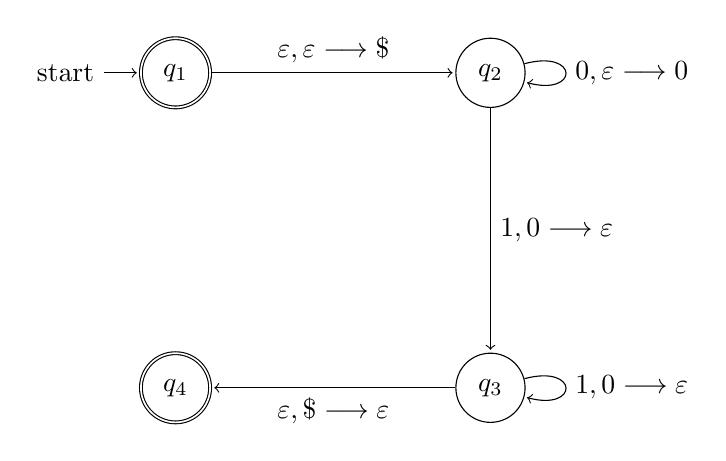
\begin{tikzpicture}[shorten >=1pt,node distance=4cm,on grid,auto] 
         
   \node[state,initial, accepting] (q_1)   {$q_1$}; 
   \node[state] (q_2) [ right=of q_1] {$q_2$};
   \node[state] (q_3) [ below=of q_2] {$q_3$};
   \node[state, accepting] (q_4) [ below=of q_1] {$q_4$};
    \path[->] 
    (q_1)
        edge  node {$ \varepsilon, \varepsilon \longrightarrow \$$} (q_2)

    (q_2) 
          edge  node {$ 1, 0  \longrightarrow \varepsilon$} (q_3)
          edge [loop right] node {$ 0, \varepsilon \longrightarrow 0$} ()
          
    (q_3)
      edge  node {$\varepsilon, \$ \longrightarrow \varepsilon$} (q_4)
      edge [loop right] node {$ 1, 0  \longrightarrow \varepsilon$} ();
\end{tikzpicture}
    
\end{enumerate}


\pagebreak

\end{document}
